\section{Casi d'uso} \label{section:casi_uso}

\subsection{Scopo}
Lo scopo di questa sezione è la descrizione in elenco di tutti i casi d'uso individuati dal gruppo, in
riferimento alle funzionalità dell'applicazione.

\subsection{Attori}
Come accordato con il proponente, la webapp deve essere usata sia dal venditore che dal cliente,
sono quindi presenti tre attori nella gerarchia: la piattaforma E-Commerce da cui parte l'ordine, Metamask\glo{}, l'utente generico.
L'utente generico ha poi due specializzazioni possibili: l'utente proprietario dell'ordine e l'utente venditore.

\begin{figure}[H]
    \centering
    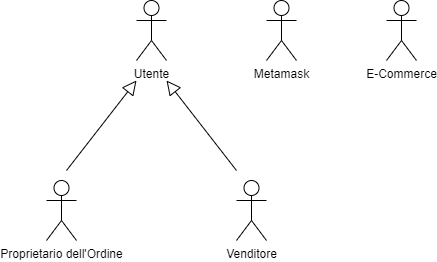
\includegraphics[scale=0.7]{immagini/UseCases-Attori.png}
    \caption{Diagramma degli Attori.}
  \end{figure}

\subsection{UC1 - Inizializzazione della Transazione}

\begin{figure}[H]
    \centering
    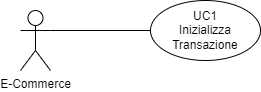
\includegraphics[scale=0.7]{immagini/UseCases-UC1.png}
    \caption{UC1.}
  \end{figure}

\begin{itemize}
    \item Attore primario: E-Commerce;
    \item Precondizioni: il sistema è raggiungibile e funzionante;
    \item Postcondizioni: la transazione viene caricata nel sistema, l'utente viene reindirizzato alla pagina di checkout;
    \item Scenario principale: L'E-Commerce delega il pagamento comunicando la somma richiesta e l'indirizzo del destinatario.
\end{itemize}

\subsection{UC2 - Tipo Pagamento}

    \begin{figure}[H]
    \centering
    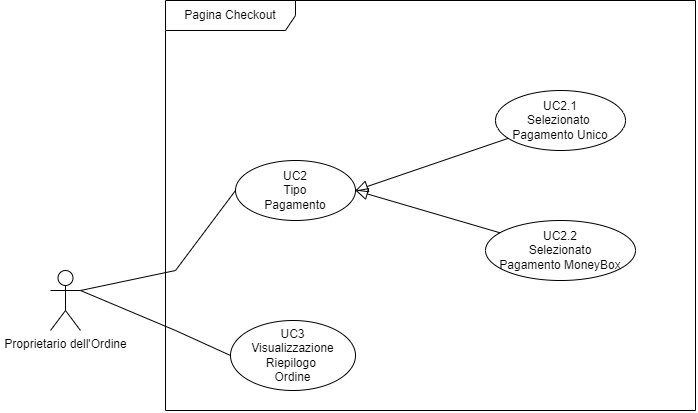
\includegraphics[scale=0.7]{immagini/UseCases-UC2-1.png}
    \caption{Pagina di checkout.}
  \end{figure}

    \begin{itemize}
    \item Attore primario: Utente proprietario dell'ordine;
    \item Precondizioni: l'E-Commerce ha iniziato la transazione [UC1];
    \item Postcondizioni: viene visualizzato il riepilogo dell'ordine e scelta la modalità di pagamento;
    \item Scenario principale: l'utente seleziona la tipologia del pagamento tra quelle disponibili;
    \item Generalizzazioni: l'utente sceglie una delle seguenti opzioni:
    \begin{itemize}
        \item pagamento unico [UC2.1].
        \item pagamento moneybox [UC2.2].
    \end{itemize}
    \end{itemize}
    \clearpage

    \subsubsection{UC2.1 - Selezionato Pagamento Unico}

    \begin{figure}[H]
    \centering
    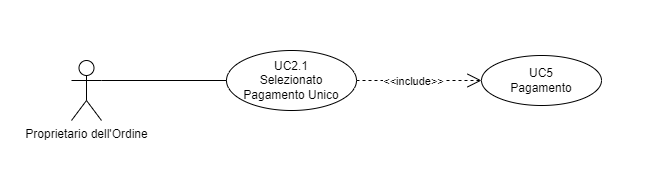
\includegraphics[scale=0.7]{immagini/UseCases-UC2-2.png}
    \caption{UC2.1.}
    \end{figure}

    \begin{itemize}
    \item Attore primario: proprietario dell'ordine;
    \item Precondizioni: l'E-Commerce ha iniziato la transazione [UC1];
    \item Postcondizioni: l'utente ha selezionato pagamento unico come metodo di pagamento e ha pagato con lo stesso;
    \item Scenario principale:
    \begin{enumerate}
        \item l'utente seleziona pagamento unico come metodo di pagamento.
        \item l'utente effettua il pagamento [UC5].
    \end{enumerate}
    \end{itemize}

    \subsubsection{UC2.2 -  Selezionato Pagamento MoneyBox}

    \begin{figure}[H]
    \centering
    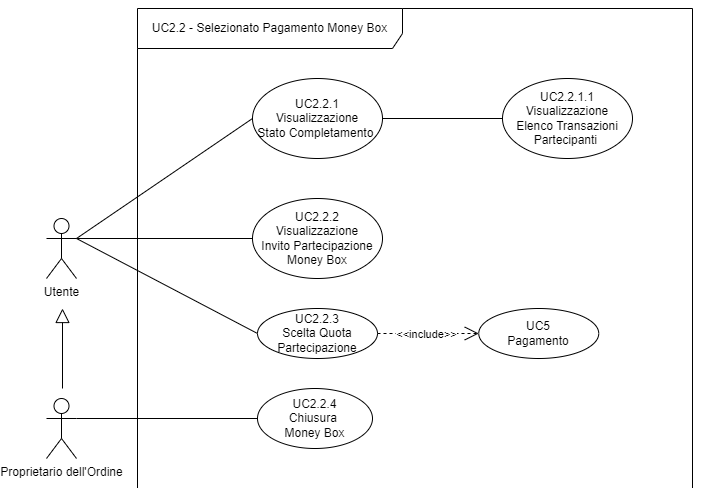
\includegraphics[scale=0.7]{immagini/UseCases-UC2-3.png}
    \caption{UC2.2 e i suoi sottocasi.}
    \end{figure}

    \begin{itemize}
    \item Attore primario: utente generico, utente proprietario dell'ordine;
    \item Precondizioni: l'E-Commerce ha iniziato la transazione [UC1];
    \item Postcondizioni: l'utente ha selezionato pagamento MoneyBox come metodo di pagamento e ha pagato con lo stesso;
    \item Scenario principale:
    \begin{enumerate}
        \item l'utente seleziona pagamento MoneyBox come metodo di pagamento;
        \item l'utente conferma la creazione della MoneyBox [UC2.2.4];
        \item l'utente visualizza lo stato di completamento [UC2.2.1];
        \item l'utente visualizza l'invito alla partecipazione della MoneyBox [UC2.2.2];
        \item l'utente, opzionalmente, partecipa alla MoneyBox [UC2.2.3];
        \item l'utente proprietario dell'ordine, opzionalmente, può chiudere una MoneyBox [UC2.2.5].
        \end{enumerate}
    \end{itemize}

    \subsubsection{UC2.2.1 - Visualizzazione Stato Completamento}

    \begin{itemize}
    \item Attore primario: utente generico;
    \item Precondizioni: l'E-Commerce ha iniziato la transazione [UC1], l'utente dispone dell'invito valido ad una MoneyBox;
    \item Postcondizioni: l'utente ha visualizzato lo stato del completamento;
    \item Scenario principale:
    \begin{enumerate}
        \item l'utente visualizza lo stato del completamento in formato percentuale e il saldo mancante;
        \item l'utente visualizza una lista delle transazioni avvenute [UC2.2.1.1].
        \end{enumerate}
    \end{itemize}

    \subsubsection{UC2.2.2 - Visualizzazione Invito Partecipazione MoneyBox}

    \begin{itemize}
    \item Attore primario: utente generico;
    \item Precondizioni: l'E-Commerce ha iniziato la transazione [UC1], l'utente dispone dell'invito valido ad una MoneyBox;
    \item Postcondizioni: l'utente ha visualizzato l'invito alla MoneyBox;
    \item Scenario principale: l'utente visualizza l'invito alla MoneyBox.
    \end{itemize}

    \subsubsection{UC2.2.3 - Scelta Quota Partecipazione}

    \begin{itemize}
    \item Attore primario: utente generico;
    \item Precondizioni: l'E-Commerce ha iniziato la transazione [UC1], l'utente dispone dell'invito valido ad una MoneyBox;
    \item Postcondizioni: l'utente ha selezionato la quota da versare e ha effettuato il pagamento;
    \item Scenario principale:
    \begin{enumerate}
        \item l'utente seleziona la quota da versare, compresa tra zero escluso e il minimo tra il saldo disponibile nel wallet e il rimanente della MoneyBox;
        \item l'utente effettua il pagamento [UC5].
    \end{enumerate}
    \end{itemize}

    \subsubsection{UC2.2.4 - Creazione MoneyBox}

    \begin{itemize}
        \item Attore primario: utente proprietario dell'ordine;
        \item Attore secondario: Metamask;
        \item Precondizioni: l'utente ha connesso il proprio Metamask [UC4] e ha selezionato il pagamento MoneyBox;
        \item Postcondizioni: l'utente ha creato una MoneyBox;
        \item Scenario principale:
        \begin{enumerate}
            \item l'utente visualizza il pop-up di Metamask;
            \item l'utente conferma l'operazione all'interno del pop-up;
            \item l'utente viene reindirizzato alla pagina con i dettagli della MoneyBox.
        \end{enumerate}
        \end{itemize}

    \subsubsection{UC2.2.5 - Chiusura MoneyBox}

    \begin{itemize}
    \item Attore primario: utente proprietario dell'ordine;
    \item Attore secondario: Metamask;
    \item Precondizioni: l'utente ha connesso il proprio Metamask [UC4];
    \item Postcondizioni: l'utente ha chiuso la MoneyBox e i fondi vengono restituiti;
    \item Scenario principale:
    \begin{enumerate}
        \item l'utente visualizza il pop-up di Metamask;
        \item l'utente conferma l'operazione all'interno del pop-up;
        \item viene annullato ogni versamento, effettuati i rimborsi e la MoneyBox viene chiusa.
    \end{enumerate}
    \end{itemize}

\subsection{UC3 - Visualizzazione Riepilogo Ordine}

\begin{figure}[H]
    \centering
    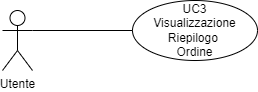
\includegraphics[scale=0.7]{immagini/UseCases-UC3.png}
    \caption{UC3.}
  \end{figure}

\begin{itemize}
    \item Attore primario: utente generico;
    \item Precondizioni: l'E-Commerce ha iniziato la transazione [UC1];
    \item Postcondizioni: l'utente ha visualizzato il riepilogo dell'ordine;
    \item Scenario principale:
    \begin{enumerate}
        \item l'utente visualizza il totale dell'ordine;
        \item l'utente visualizza l'indirizzo del venditore.
    \end{enumerate}
\end{itemize}

\subsection{UC4 - Connessione Metamask}

\begin{figure}[H]
    \centering
    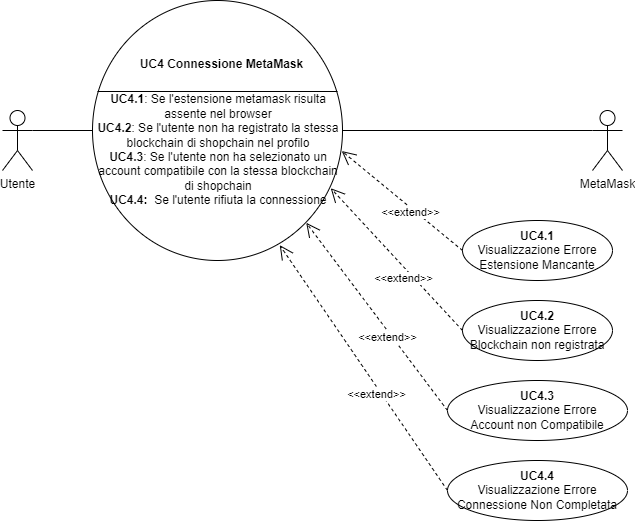
\includegraphics[scale=0.7]{immagini/UseCases-UC4.png}
    \caption{UC4.}
  \end{figure}

\begin{itemize}
    \item Attore primario: utente generico;
    \item Precondizioni: il sistema è raggiungibile e funzionante;
    \item Postcondizioni: l'utente ha connesso Metamask a ShopChain;
    \item Scenario principale:
    \begin{enumerate}
        \item l'utente visualizza il pop-up di Metamask per la connessione a ShopChain;
        \item l'utente autorizza la connessione a ShopChain.
    \end{enumerate}
    \item Estensioni:
    \begin{enumerate}
        \item Nel caso in cui l'estensione Metamask risultasse assente nel browser:
        \begin{itemize}
            \item la connessione non ha successo;
            \item viene visualizzato errore estensione mancante [UC4.1].
        \end{itemize}
        \item Nel caso in cui l'utente abbia connesso il proprio wallet ma non abbia configurato la stessa blockchain di ShopChain:
        \begin{itemize}
            \item la connessione non viene completata;
            \item viene visualizzato errore blockchain non registrata [UC4.2].
        \end{itemize}
        \item Nel caso in cui l'utente abbia configurato la stessa blockchain di ShopChain ma non selezionato un account compatibile:
        \begin{itemize}
            \item la connessione non viene completata;
            \item viene visualizzato errore account non compatibile [UC4.3].
        \end{itemize}
        \item Nel caso l'utente rifiuti la connessione, visualizza errore connessione non completata [UC4.4].
    \end{enumerate}
\end{itemize}

\subsubsection{UC4.1 - Visualizzazione Errore Estensione Mancante}

\begin{itemize}
    \item Attore primario: utente generico;
    \item Precondizioni: l'utente utilizza un browser sprovvisto di estensione Metamask;
    \item Postcondizioni: l'utente ha visualizzato l'errore e la connessione fallisce;
    \item Scenario principale: 
    \begin{enumerate}
        \item l'utente visualizza un messaggio di errore per mancata connessione;
        \item l'utente viene invitato a scaricare l'estensione Metamask;
        \item l'utente clicca ”OK” per continuare.
    \end{enumerate}
\end{itemize}

\subsubsection{UC4.2 - Visualizzazione Errore Blockchain non registrata}

\begin{itemize}
    \item Attore primario: utente generico;
    \item Precondizioni:l'utente ha connesso il proprio wallet ma non ha configurato la stessa blockchain di ShopChain;
    \item Postcondizioni: l'utente ha visualizzato l'errore e la connessione fallisce;
    \item Scenario principale:
    \begin{enumerate}
        \item l'utente visualizza un messaggio di errore per mancata connessione;
        \item l'utente visualizza i dati per configurare la blockchain;
        \item l'utente clicca ”OK” per continuare.
    \end{enumerate}
\end{itemize}

\subsubsection{UC4.3 - Visualizzazione Errore account non compatibile}

\begin{itemize}
    \item Attore primario: utente generico;
    \item Precondizioni: l'utente ha configurato la stessa blockchain di ShopChain ma non ha selezionato un account compatibile;
    \item Postcondizioni: l'utente ha visualizzato l'errore e la connessione fallisce;
    \item Scenario principale:
    \begin{enumerate}
        \item l'utente visualizza un messaggio di errore per mancata connessione;
        \item l'utente viene invitato a cambiare account o a registrare un account compatibile;
        \item l'utente clicca ”OK” per continuare.
    \end{enumerate}
\end{itemize}

\subsubsection{UC4.4 - Visualizzazione Errore connessione non completata}

\begin{itemize}
    \item Attore primario: utente generico;
    \item Precondizioni: l'utente rifiuta la connessione;
    \item Postcondizioni: l'utente ha visualizzato l'errore e la connessione fallisce;
    \item Scenario principale:
    \begin{enumerate}
        \item l'utente visualizza un messaggio di errore per mancata connessione;
        \item l'utente viene invitato a ritentare;
        \item l'utente clicca ”OK” per continuare.
    \end{enumerate}
\end{itemize}

\subsection{UC5 - Pagamento}

\begin{figure}[H]
    \centering
    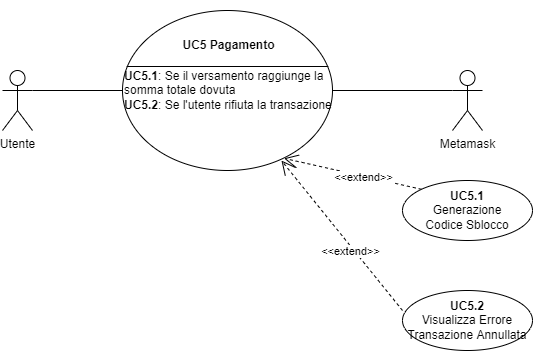
\includegraphics[scale=0.7]{immagini/UseCases-UC5.png}
    \caption{UC5.}
  \end{figure}

\begin{itemize}
    \item Attore primario: utente generico;
    \item Attore secondario: Metamask;
    \item Precondizioni: l'utente ha scelto il Tipo di Pagamento [UC2], l'utente ha connesso il proprio wallet tramite Metamask [UC4];
    \item Postcondizioni: l'utente ha effettuato il pagamento;
    \item Scenario principale:
    \begin{enumerate}
        \item l'utente visualizza il pop-up di Metamask con i dettagli della transazione, solo in caso di saldo sufficiente;
        \item l'utente autorizza la transazione;
        \item l'utente visualizza un messaggio di conferma di avvenuto pagamento.
    \end{enumerate}
    \item Estensioni:
    \begin{enumerate}
        \item Nel caso l'utente rifiuti il pagamento:
        \begin{itemize}
            \item la transazione viene annullata;
            \item l'utente visualizza errore transazione annullata [UC5.2].
        \end{itemize}
        \item Nel caso venisse raggiunta la somma totale dovuta, viene generato e mostrato il codice di sblocco [UC5.1].
    \end{enumerate}
\end{itemize}

\subsubsection{UC5.1 - Generazione Codice di Sblocco}

\begin{itemize}
    \item Attore primario: utente generico;
    \item Precondizioni: il versamento raggiunge la somma totale dovuta;
    \item Postcondizioni: l'utente ha visualizzato il codice di sblocco;
    \item Scenario principale:
    \begin{enumerate}
        \item viene generato il codice di sblocco;
        \item l'utente visualizza il codice di sblocco.
    \end{enumerate}
\end{itemize}

\subsubsection{UC5.2 - Visualizzazione errore transazione annullata}

\begin{itemize}
    \item Attore primario: utente generico;
    \item Precondizioni: la transazione non è andata a buon fine;
    \item Postcondizioni: l'utente ha visualizzato l'errore e la transazione fallisce;
    \item Scenario principale:
    \begin{enumerate}
        \item l'utente visualizza un messaggio di errore per rifiuto della transazione;
        \item l'utente clicca ”OK” per continuare.
    \end{enumerate}
\end{itemize}

\subsection{UC6 - Sblocco Ordine}

\begin{figure}[H]
    \centering
    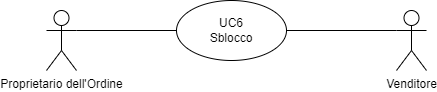
\includegraphics[scale=0.7]{immagini/UseCases-UC6.png}
    \caption{UC6.}
  \end{figure}

\begin{itemize}
    \item Attore primario: utente proprietario dell'ordine;
    \item Attore secondario: utente venditore, Metamask;
    \item Precondizioni: il sistema ha generato il codice di sblocco [UC5.2];
    \item Postcondizioni: l'utente proprietario ha sbloccato l'ordine e il denaro è stato trasferito all'utente venditore;
    \item Scenario principale:
    \begin{enumerate}
        \item l'utente inserisce il codice di sblocco;
        \item l'utente conferma la transazione sul pop-up Metamask;
        \item il sistema trasferisce il denaro sul wallet dell'utente venditore.
    \end{enumerate}
\end{itemize}

\subsection{UC7 - Visualizzazione Transazioni}

\begin{figure}[H]
    \centering
    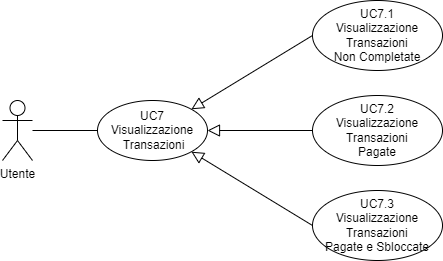
\includegraphics[scale=0.7]{immagini/UseCases-UC7.png}
    \caption{UC7.}
  \end{figure}

\begin{itemize}
    \item Attore primario: utente generico;
    \item Precondizioni: il sistema è raggiungibile e funzionante;
    \item Postcondizioni: l'utente ha selezionato lo stato delle transazioni che vuole visualizzare;
    \item Scenario principale: l'utente sceglie lo stato delle transazioni da visualizzare tra quelli disponibili;
    \item Generalizzazioni: l'utente sceglie una delle seguenti opzioni:
    \begin{itemize}
        \item visualizza transazioni non completate [UC7.1];
        \item visualizza transazioni pagate [UC7.2];
        \item visualizza transazioni pagate e sbloccate [UC7.3].
    \end{itemize}
\end{itemize}

\subsubsection{UC7.1 - Visualizza Transazioni Non Completate}

\begin{itemize}
    \item Attore primario: utente venditore;
    \item Precondizioni: l'utente ha selezionato visualizza transazioni non completate;
    \item Postcondizioni: l'utente ha visualizzato la lista di transazioni non completate;
    \item Scenario principale: l'utente visualizza la lista di transazioni non completate.
\end{itemize}

\subsubsection{UC7.2 - Visualizza Transazioni Pagate}

\begin{itemize}
    \item Attore primario: utente venditore;
    \item Precondizioni: l'utente ha selezionato visualizza transazioni pagate;
    \item Postcondizioni: l'utente ha visualizzato la lista di transazioni pagate;
    \item Scenario principale: l'utente visualizza la lista di transazioni pagate.
\end{itemize}

\subsubsection{UC7.3 - Visualizza Transazioni Pagate e Sbloccate}

\begin{itemize}
    \item Attore primario: utente venditore;
    \item Precondizioni: l'utente ha selezionato visualizza transazioni pagate e sbloccate;
    \item Postcondizioni: l'utente ha visualizzato la lista di transazioni pagate e sbloccate;
    \item Scenario principale: l'utente visualizza la lista di transazioni pagate e sbloccate.
\end{itemize}
\clearpage
